\begin{frame}
    \frametitle{Bitcoin Mania}
    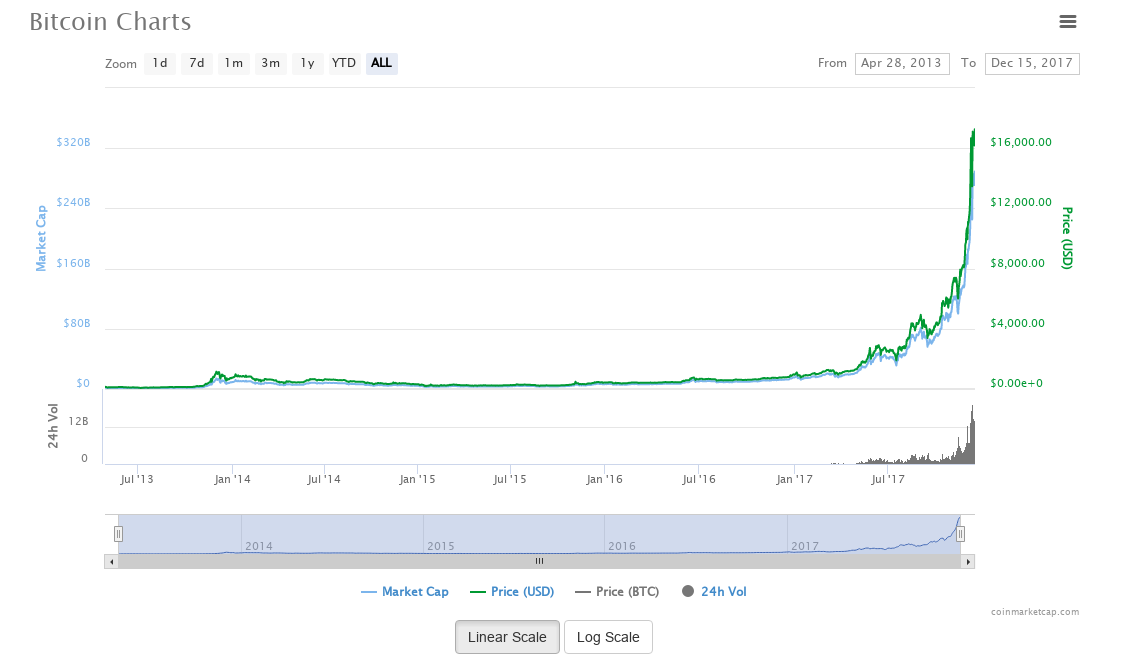
\includegraphics[scale=0.3]{bitcoin-usd-prices.png}
\end{frame}

\begin{frame}
    \frametitle{Bitcoin Mania}
    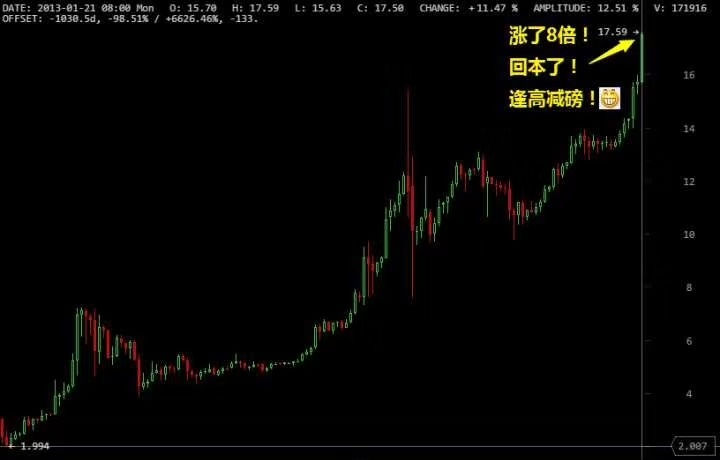
\includegraphics[scale=0.3]{bitcoin-invest0.jpg}
\end{frame}

\begin{frame}
    \frametitle{Bitcoin Mania}
    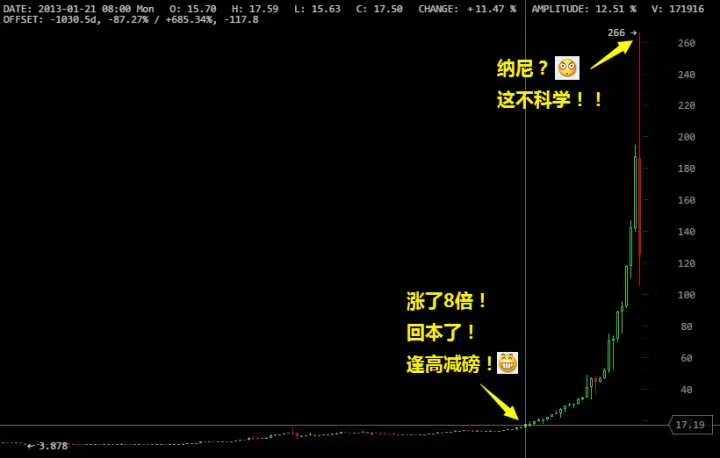
\includegraphics[scale=0.3]{bitcoin-invest1.jpg}
\end{frame}

\begin{frame}
    \frametitle{Bitcoin Mania}
    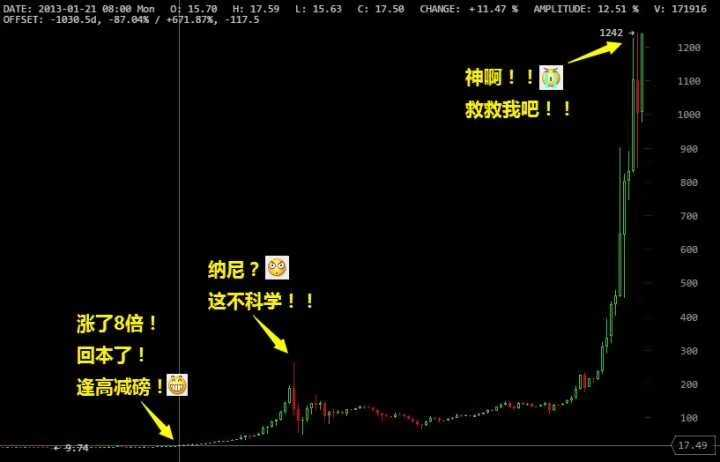
\includegraphics[scale=0.3]{bitcoin-invest2.jpg}
\end{frame}

\begin{frame}
    \frametitle{Bitcoin Mania}
    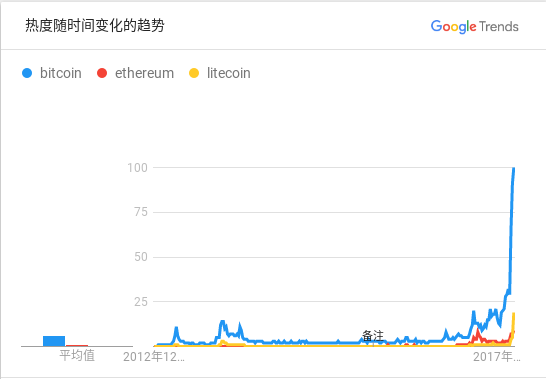
\includegraphics[scale=0.4]{bitcoin-google-trends.png}
\end{frame}

\begin{frame}
    \frametitle{Bitcoin Mania}
    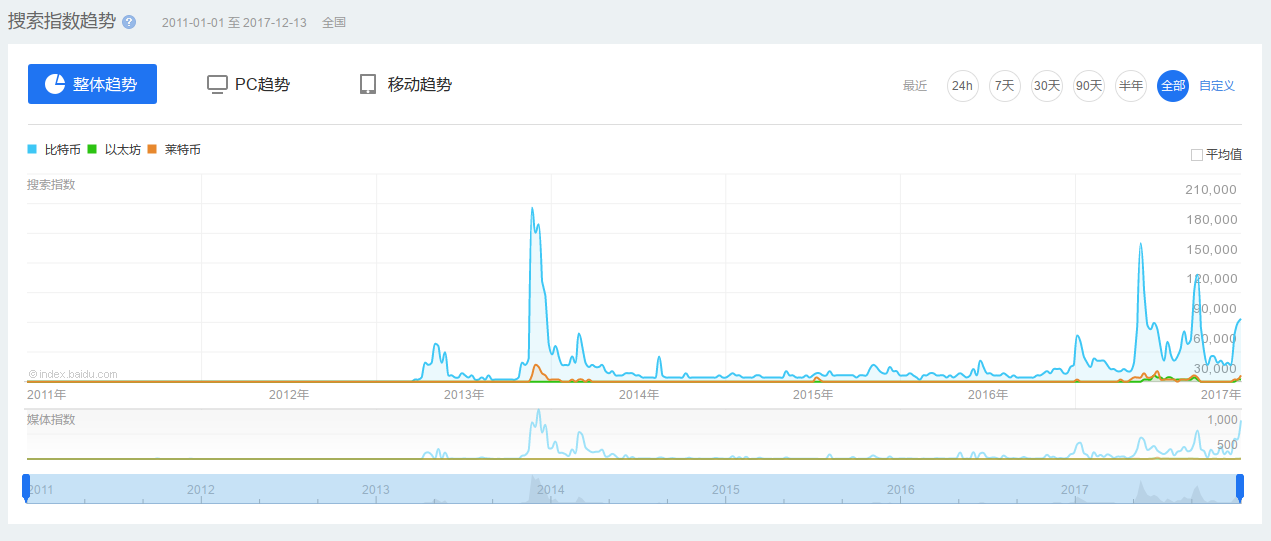
\includegraphics[scale=0.26]{bitcoin-baidu-index.png}
\end{frame}

\begin{frame}
    \frametitle{BlockChain}
    \begin{block}{国务院2016年十三五报告}
        “十三五”时期,全球信息化发展面临的环境、条件和内涵正发生深刻变化 \ldots
        信息技术创新代际周期大幅缩短,创新活力、集聚效应和应用潜能裂变式释放,更快速度、更广范围、更深程度地引发新一轮科技革命和产业变革。物联网、云计算、大数据、人工智能、机器深度学习、\alert{区块链}、生物基因工程等新技术驱动网络空间从人人互联向万物互联演进,数字化、网络化、智能化服务将无处不在。现实世界和数字世界日益交汇融合,全球治理体系面临深刻变革。全球经济体普遍把加快信息技术创新、最大程度释放数字红利,作为应对“后金融危机”时代增长不稳定性和不确定性、深化结构性改革和推动可持续发展的关键引擎。
    \end{block}
\end{frame}

\begin{frame}
    \frametitle{Barter System}
    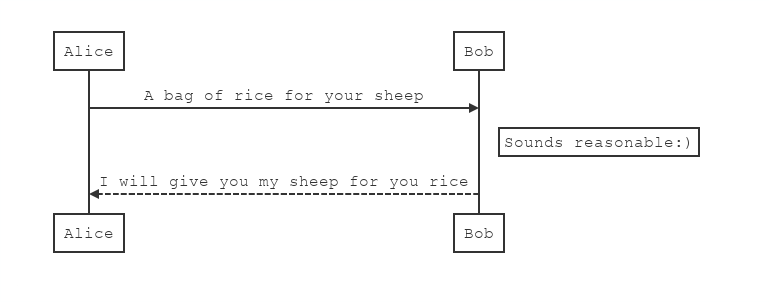
\includegraphics[scale=0.4]{barter-system.png}
\end{frame}

\begin{frame}
    \frametitle{Gold Money}
    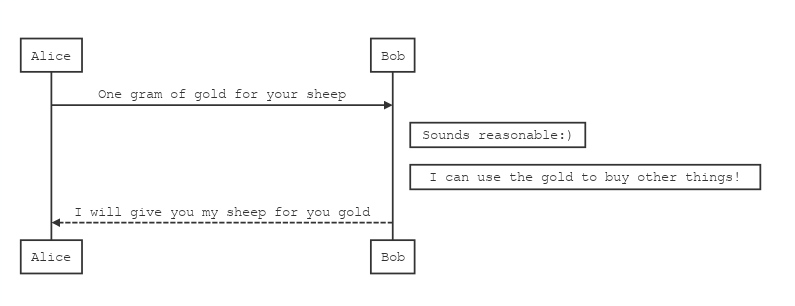
\includegraphics[scale=0.4]{gold-money.png}
\end{frame}

\begin{frame}
    \frametitle{Paper Money}
    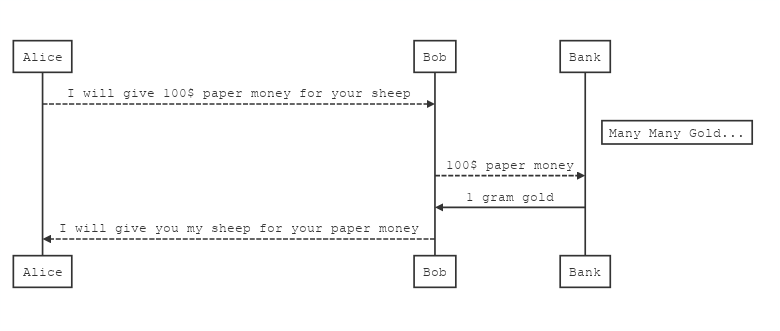
\includegraphics[scale=0.4]{paper-money.png}
\end{frame}

\begin{frame}
    \frametitle{Central Banking}
    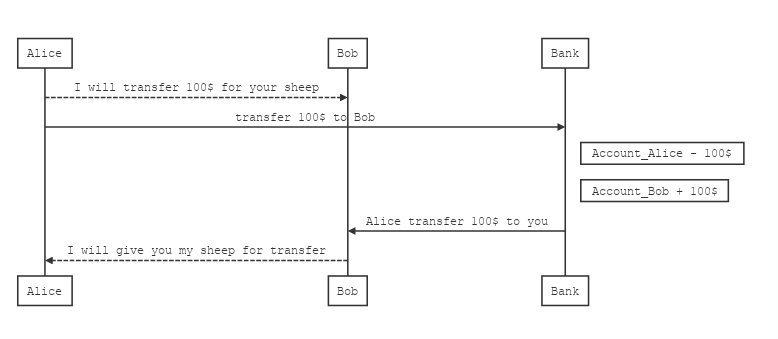
\includegraphics[scale=0.4]{central-banking.png}
\end{frame}

\begin{frame}
    \frametitle{Nature of Money}
    \textbf{What is Money?}
    \begin{itemize}
        \item \textbf{Medium of exchange}
            \begin{itemize}
                \item Standard object used in exchanging goods and services
            \end{itemize}
        \item \textbf{Unit of account}
            \begin{itemize}
                \item Standard unit used for quoting prices
            \end{itemize}
        \item \textbf{Store of value}
            \begin{itemize}
                \item Store wealth from one point in time to another
            \end{itemize}
    \end{itemize}
\end{frame}

\begin{frame}
    \frametitle{What is Bitcoin?}
    \begin{block}{Wikipedia}
        Bitcoin is the first \alert{decentralized digital cryptocurrency}, as the \alert{worldwide payment system} works without a central bank or single administrator. The network is \alert{peer-to-peer} and transactions take place between users directly through the use of cryptography, without an intermediary. These \alert{transactions} are verified by network nodes, which called \alert{mining} and recorded in a \alert{public distributed ledger} called a \alert{blockchain}. Bitcoin was invented by an unknown person or group of people under the name \alert{Satoshi Nakamoto} and released as \alert{open-source software} in 2009.
    \end{block}
\end{frame}

\begin{frame}
    \frametitle{Video}
    \begin{center}
        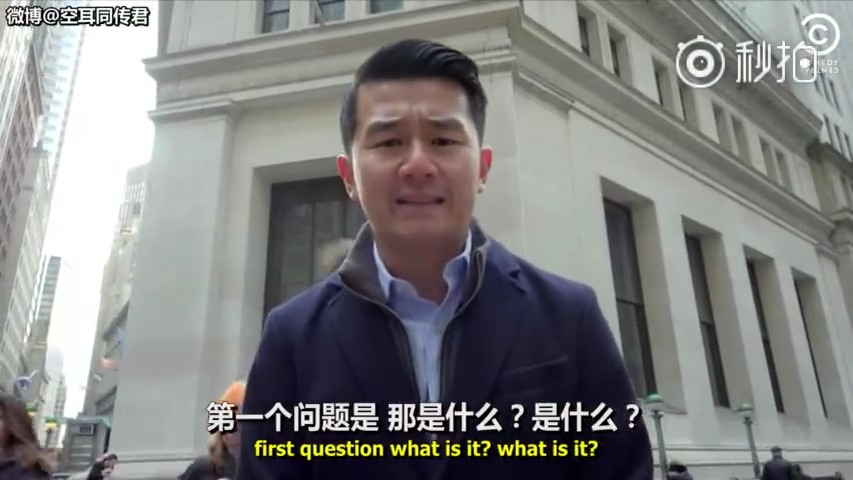
\includegraphics[scale=0.35]{what-it-it.jpg} \\
        \href{run:cryptocurrency.mp4}{\textbf{Bitcoin, What is it?}}
    \end{center}
\end{frame}

\begin{frame}
    \frametitle{Bitcoin Overview}
    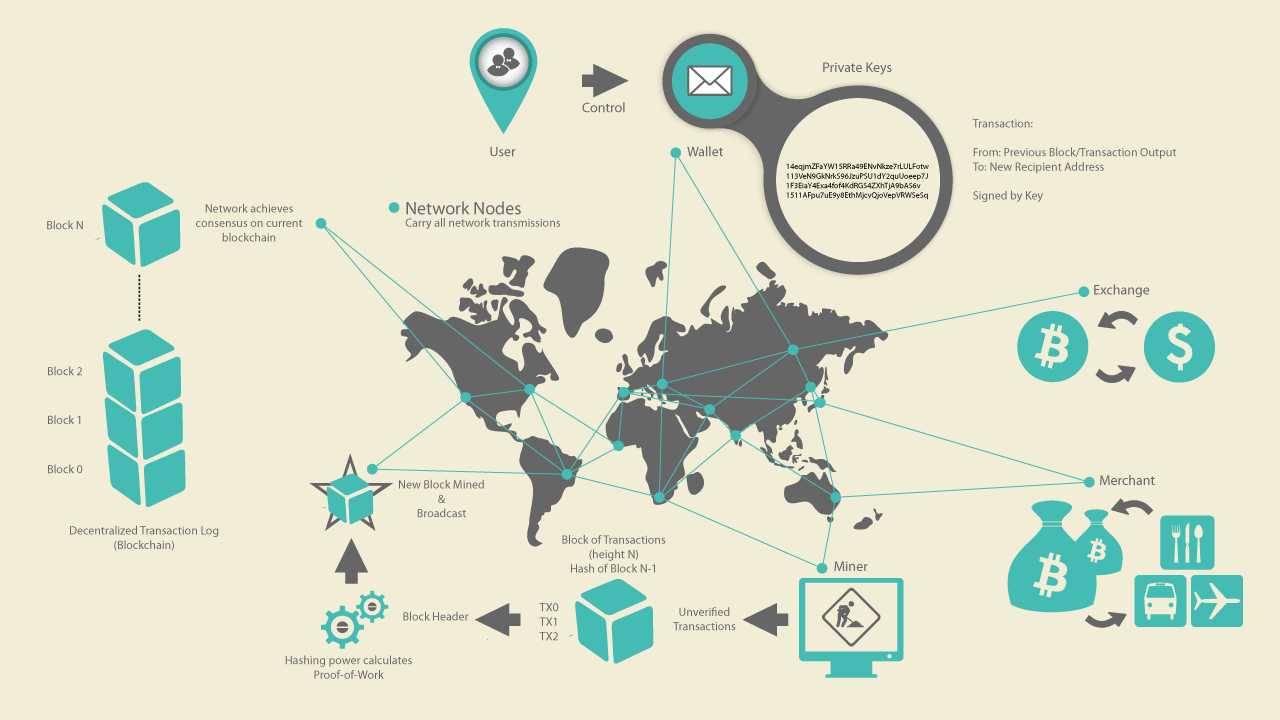
\includegraphics[scale=1]{mbc2_0201.png}
\end{frame}

\begin{frame}[fragile]
    \frametitle{Buying a cup of coffee}
    Alice buyes a cup of coffee at Bob's coffee shop, paying with BTC.
    \begin{columns}
        \begin{column}{0.6\textwidth}
            \begin{lstlisting}[language=Python]
bitcoin:1GdK9UzpHBzqzX2A9JFP3Di4weBwqgmoQA?\
amount=0.015&\
label=Bob%27s%20Cafe&\
message=Purchase%20at%20Bob%27s%20Cafe

Components of the URL
A bitcoin address: "1GdK9UzpHBzqzX2A9JFP3Di4weBwqgmoQA"
The payment amount: "0.015"
A label for the recipient address: "Bob's Cafe"
A description for the payment: "Purchase at Bob's Cafe"
            \end{lstlisting}
        \end{column}
        \begin{column}{0.3\textwidth}
            
\includegraphics[scale=1]{mbc2_0202.png}
        \end{column}
    \end{columns}
\end{frame}

\begin{frame}
    \begin{center}
        \textbf{\alert{\huge{Q \& A}}}
    \end{center}
\end{frame}

\begin{frame}
    \frametitle{Bitcoin: Challenges}
    \begin{itemize}
        \item \textbf{Creation of a virtual coin}
            \begin{itemize}
                \item How is it created in the first place?
                \item How do you prevent inflation?
            \end{itemize}
        \item \textbf{Validation}
            \begin{itemize}
                \item Is the coin legit? \alert{(Proof-Of-Work)}
                \item How do you prevent a coin from \alert{double-spending}?
            \end{itemize}
        \item \textbf{Buyer and seller protection in online transactions}
            \begin{itemize}
                \item Buyer pays, but the seller doesn't deliver
                \item Seller delivers, buyer pays, but the buyer makes a claim
            \end{itemize}
        \item \textbf{Trust on third party}
            \begin{itemize}
                \item Rely on proof instead of trust
                \item Verifiable by everyone
                \item No central bank
            \end{itemize}
    \end{itemize}
\end{frame}

\begin{frame}
    \frametitle{CryptoCurrency}
    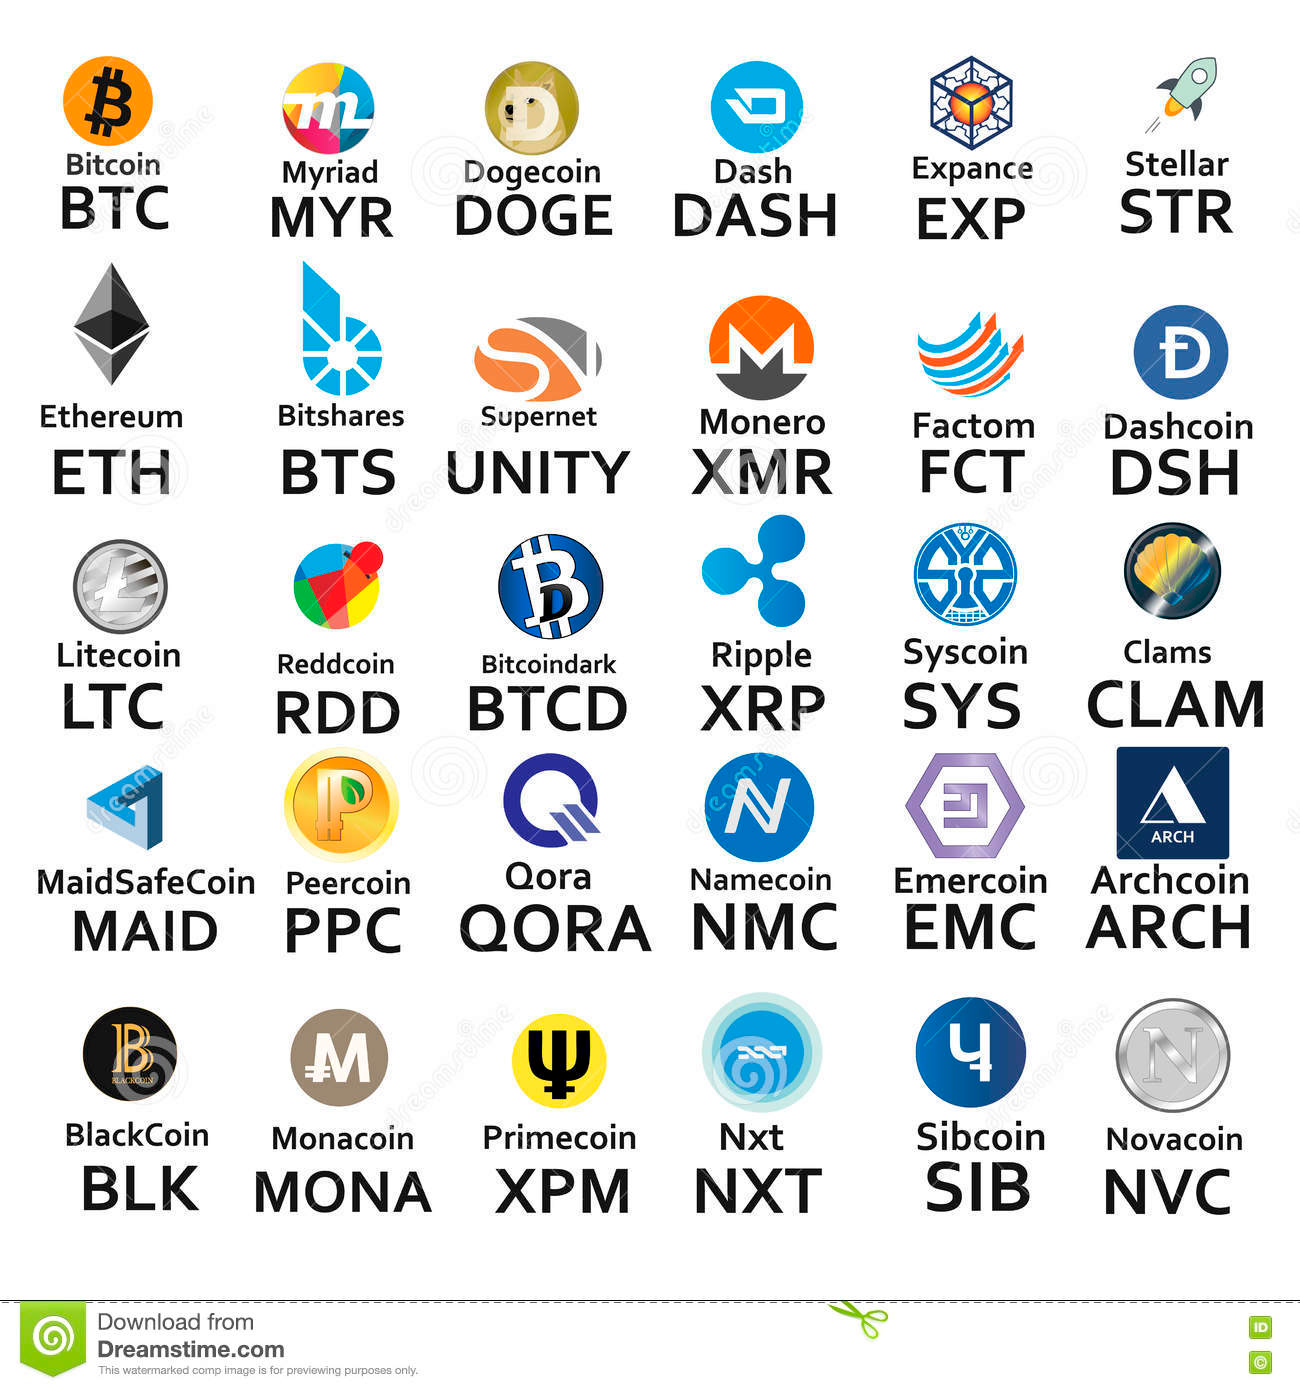
\includegraphics[scale=0.16]{cryptocurrency.png}
\end{frame}

\begin{frame}[fragile]
    \frametitle{Bitcoin Overview}
    \begin{lstlisting}[language=JavaScript]
function mine()
{
    while (true)
    {
        longestChain = getLongestValidChain();

        // A number that changes every time, so that you don't waste time
        // trying to calculate a valid blockHash with the same input.
        nonce = getNewNonce();

        currentTXs = getUnconfirmedTransactionsFromNetwork();
        newBlock = getNewBlock(longestChain, currentTX, nonce);

        // Hash function, and this is what all the *mining machines* are doing
        blockHash = sha256(newBlock)

        if (meetRequirements(blockHash))
        {
            broadcast(newBlock)
            // now the height of the block chain is incremented by 1
            // if the new block is accepted by other peers
            // and all the TXs in the new block are "confirmed"
        }
    }
}
    \end{lstlisting}
\end{frame}

\begin{frame}[fragile]
    \frametitle{Bitcoin Overview}
    \begin{lstlisting}[language=JavaScript]
function sendBTC(amount)
{
    sourceTXs = pickConfirmedTransactionsToBeSpent(amount);
    tx = generateTX(sourceTx, targetAddrs, amount, fee);
    signedTx = sign(tx, privateKeysOfAllInputAddress);
    broadcast(signedTx);
}
    \end{lstlisting}
\end{frame}

